\documentclass[11pt,letterpaper]{article}
\usepackage[lmargin=1in,rmargin=1in,tmargin=1in,bmargin=1in]{geometry}
\usepackage{../style/homework}
\usepackage{../style/commands}
\setbool{quotetype}{true} % True: Side; False: Under
\setbool{hideans}{false} % Student: True; Instructor: False

\newcommand{\blank}[1]{\underline{\hspace{#1}}} % Blank Underline

% -------------------
% Content
% -------------------
\begin{document}

\homework{10: Due 11/10}{Matrices act. They don't just sit there.}{Gilbert Strang}

% Problem 1
\problem{10} Showing all your work, compute the following:
	\begin{enumerate}[(a)]
	\item $\displaystyle \sum_{k=0}^5 (5k - 3)$
	\item $\displaystyle \sum_{\substack{k= -2 \\ k \neq 0}}^3 \dfrac{k + 1}{k}$
	\item $\displaystyle \prod_{j=1}^4 2j$
	\item $\displaystyle \prod_{n=2}^\infty \left(1 - \dfrac{1}{n^2} \right)$ \quad [Hint: Combine terms, factor, then write out some terms.]
	\item $\displaystyle \sum_{k=1}^\infty \dfrac{1}{k^2 + 3k}$ \quad [Hint: Use partial fractions, then write out some terms.]
	\end{enumerate} \pspace

\sol 
\begin{enumerate}[(a)]
\item 
	\[
	\begin{aligned}
	\sum_{k=0}^5 (5k - 3)&= (5 \cdot 0 - 3) + (5 \cdot 1 - 3) + (5 \cdot 2 - 3) + (5 \cdot 3 - 3) + (5 \cdot 4 - 3) + (5 \cdot 5 - 3) \\
	&= -3 + 2 + 7 + 12 + 17 + 22 \\
	&= 57
	\end{aligned}
	\]
	
	\begin{center} {\itshape OR} \end{center}
	
We use the fact that $\displaystyle \sum_{k=a}^b c= (b - a + 1)c$ and $\displaystyle \sum_{k=0}^n k= \frac{k(k + 1)}{2}$, where $c \in \mathbb{R}$ is a constant. 

	\[
	\begin{aligned}
	\sum_{k=0}^5 (5k - 3)= \sum_{k=0}^5 5k - \sum_{k=0}^5 3= 5 \sum_{k=0}^5 k - \sum_{k=0}^5 3= 5 \cdot \dfrac{n(n + 1)}{2} \bigg|_{n=5} - (5 - 0 + 1)3= 5 \cdot \dfrac{5(6)}{2} - 6 \cdot 3= 57
	\end{aligned}
	\] \pspace

\item 
	\[
	\sum_{\substack{k= -2 \\ k \neq 0}}^3 \dfrac{k + 1}{k}= \dfrac{-2 + 1}{-2} + \dfrac{-1 + 1}{-1} + \dfrac{1 + 1}{1} + \dfrac{2 + 1}{2} + \dfrac{3 + 1}{3}= \dfrac{1}{2} + 0 + 2 + \dfrac{3}{2} + \dfrac{4}{3}= \dfrac{16}{3}
	\]
\end{enumerate}

\newpage 
\begin{center} {\itshape --- Continued Space for Problem~1 ---} \end{center} \pspace

\begin{enumerate}
\item[(c)] 
	\[
	\prod_{j=1}^4 2j= 2(1) \cdot 2(2) \cdot 2(3) \cdot 2(4)= 2 \cdot 4 \cdot 6 \cdot 8= 384
	\]
		\begin{center} {\itshape OR} \end{center}
	\[
	\prod_{j=1}^4 2j= 2^{4 - 1 + 1} \prod_{j=1}^4 j= 2^4 \cdot \big( 1 \cdot 2 \cdot 3 \cdot 4 \big)= 2^4 \cdot 4!= 16 \cdot 24= 384
	\] \pspace

\item[(d)] 
	\[
	\begin{aligned}
	\prod_{n=2}^\infty \left(1 - \dfrac{1}{n^2} \right)&= \prod_{n=2}^\infty \left( \dfrac{n^2 - 1}{n^2} \right) \\
	&= \prod_{n=2}^\infty \left( \dfrac{(n - 1)(n + 1)}{n \cdot n} \right) \\
	&= \dfrac{1 \cdot 3}{2 \cdot 2} \cdot \dfrac{2 \cdot 4}{3 \cdot 3} \cdot \dfrac{3 \cdot 5}{4 \cdot 4} \cdot \dfrac{4 \cdot 6}{5 \cdot 5} \cdots \\
	&= \dfrac{1 \cdot 3}{2 \cdot \cancel{2}} \cdot \dfrac{\cancel{2} \cdot 4}{3 \cdot \cancel{3}} \cdot \dfrac{\cancel{3} \cdot 5}{4 \cdot \cancel{4}} \cdot \dfrac{\cancel{4} \cdot 6}{5 \cdot \cancel{5}} \cdots \\
	&= \dfrac{1 \cdot 3}{2} \cdot \dfrac{4}{3} \cdot \dfrac{5}{4} \cdot \dfrac{6}{5} \cdots \\
	&= \dfrac{1 \cdot \cancel{3}}{2} \cdot \dfrac{\cancel{4}}{\cancel{3}} \cdot \dfrac{\cancel{5}}{\cancel{4}} \cdot \dfrac{\cancel{6}}{\cancel{5}} \cdots \\
	&= \dfrac{1}{2}
	\end{aligned}
	\]
Alternatively, to make this argument rigorous, we can define $\displaystyle a_k:= \prod_{n=2}^k \left(1 - \dfrac{1}{n^2} \right)$. Using the `cancellation trick' from above, we can observe that\dots
	\[
	\begin{aligned}
	a_k&:= \prod_{n=2}^k \left(1 - \dfrac{1}{n^2} \right) \\
	&= \prod_{n=2}^k \dfrac{(n - 1)(n + 1)}{n \cdot n} \\
	&= \dfrac{1 \cdot 3}{2 \cdot 2} \cdot \dfrac{2 \cdot 4}{3 \cdot 3} \cdot \dfrac{3 \cdot 5}{4 \cdot 4} \cdot \cdots \cdot \dfrac{(k - 2) \cdot k}{(k -1) \cdot (k - 1)} \cdot \dfrac{(k - 1)(k + 1)}{k \cdot k} \\
	&= \dfrac{1 \cdot \cancel{3}}{2 \cdot \cancel{2}} \cdot \dfrac{\cancel{2} \cdot 4}{\cancel{3} \cdot \cancel{3}} \cdot \dfrac{\cancel{3} \cdot \cancel{5}}{\cancel{4} \cdot \cancel{4}} \cdot \cdots \cdot \dfrac{\cancel{(k - 2)} \cdot \cancel{k}}{\cancel{(k -1)} \cdot \cancel{(k - 1)}} \cdot \dfrac{\cancel{(k - 1)}(k + 1)}{\cancel{k} \cdot k} \\	
	&= \dfrac{1}{2} \cdot \dfrac{k + 1}{k} \\
	&= \dfrac{1}{2} \left(1 + \dfrac{1}{k} \right)
	\end{aligned}
	\]
But then we have\dots
	\[
	\prod_{n=2}^\infty \left(1 - \dfrac{1}{n^2} \right)= \lim_{k \to \infty} a_k= \lim_{k \to \infty} \dfrac{1}{2} \left(1 + \dfrac{1}{k} \right)= \dfrac{1}{2}\; (1 + 0)= \dfrac{1}{2}
	\]

	\begin{center} {\itshape OR} \end{center}

Assume that $\displaystyle L= \lim_{N \to \infty} \prod_{n=2}^N \left(1 - \frac{1}{n^2} \right)$.\footnote{The limit exists so that $L$ is well-defined: let $a_N= \prod_{n=2}^N \left(1 - \frac{1}{n^2} \right)$. Now $1 < n^2$ for $n > 1$, so that $1> \frac{1}{n^2}$ which implies $1- \frac{1}{n^2} > 0$ for $n > 1$. Furthermore, $1 - \frac{1}{n^2} < 1$, so that $0 < 1 - \frac{1}{n^2} < 1$. Using this work and a simple induction argument, one can show that $0 < a_N < 1$ for all $N$. Moreover, $\{ a_N \}$ is a decreasing sequence because $a_{N + 1}= a_N \left(1 - \frac{1}{N + 1} \right) < a_N \cdot 1= a_N$. But then $\{ a_N \}$ is a bounded, decreasing sequence. Therefore, by the Monotone Convergence Theorem, $\{ a_N \}$ converges.} Recall the following telescoping series:
	\[
	\hspace{-2.5cm}
	\begin{gathered}
	\sum_{k=a}^b \left( \ln(k + 1) - \ln k \right) \\[0.3cm]
	=\big( \ln(a + 1) - \ln a \big) + \big( \ln(a + 2) - \ln(a + 1) \big) + \big( \ln(a + 3) - \ln(a + 2) \big) + \cdots + \big( \ln(b) - \ln(b - 1) \big) + \big( \ln(b + 1) - \ln b \big) \\[0.3cm]
	=\big( \cancel{\ln(a + 1)} - \ln a \big) + \big( \cancel{\ln(a + 2)} - \cancel{\ln(a + 1)} \big) + \big( \cancel{\ln(a + 3)} - \cancel{\ln(a + 2)} \big) + \cdots + \big( \cancel{\ln(b)} - \cancel{\ln(b - 1)} \big) + \big( \ln(b + 1) - \cancel{\ln b} \big) \\[0.3cm]
	= -\ln a + \ln(b + 1) \\[0.3cm]
	= \ln(b + 1) - \ln a
	\end{gathered}
	\]
Examining $\ln(L)$,\footnote{Using the Monotone Convergence Theorem, we know that $\inf a_N= \lim_{a_N}$. A priori, we need worry that $\inf a_N= 0$. But we can see from the `cancellation trick' from previous work that $a_N= \frac{1}{2} \left(1 + \frac{1}{N} \right) > \frac{1}{2}$. Therefore, $\inf a_N \geq \frac{1}{2}$, so that $\ln(L)$ is well-defined.} making use of the continuity of $\ln x$,\footnote{For continuous functions, $f(x)$, we have $\lim f(x_n)= f( \lim x_n)$.}, and making use of the telescoping series above, we can observe\dots
	\[
	\begin{aligned}
	\ln L&= \ln \left( \lim_{N \to \infty} \prod_{n=2}^N \left(1 - \frac{1}{n^2} \right) \right) \\
	&= \lim_{N \to \infty} \ln \left( \prod_{n=2}^N \left(1 - \frac{1}{n^2} \right) \right) \\
	&= \lim_{N \to \infty} \sum_{k=2}^N \ln \left(1 - \frac{1}{n^2} \right) \\
	&= \lim_{N \to \infty} \sum_{k=2}^N \ln \left( \dfrac{n^2 - 1}{n^2} \right) \\
	&= \lim_{N \to \infty} \sum_{k=2}^N \big( \ln(n^2 - 1) - \ln(n^2) \big) \\
	&= \lim_{N \to \infty} \sum_{k=2}^N \big( \ln \big( (n + 1)(n - 1) \big) - 2\ln(n) \big) \\
	\end{aligned}
	\]
	\[
	\begin{aligned}
	&= \lim_{N \to \infty} \sum_{k=2}^N \big( \ln(n + 1) + \ln(n - 1) - 2\ln(n) \big) \\
	&= \lim_{N \to \infty} \sum_{k=2}^N \big( \ln(n + 1) - \ln n + \ln(n - 1) - \ln(n) \big) \\
	&= \lim_{N \to \infty} \left( \sum_{k=2}^N \big( \ln(n + 1) - \ln n \big) + \sum_{k=2}^N \big( \ln(n - 1) - \ln(n) \big) \right) \\
	&= \lim_{N \to \infty} \left( \sum_{k=2}^N \big( \ln(n + 1) - \ln n \big) - \sum_{k=2}^N \big( \ln(n) - \ln(n - 1) \big) \right) \\
	&= \lim_{N \to \infty} \left( \big( \ln(N+1) - \ln 2 \big) - \big( \ln N - \ln(2 - 1) \big) \right) \\
	&= \lim_{N \to \infty} \left( \big( \ln(N+1) - \ln 2 \big) - \big( \ln N - \ln 1 \big) \right) \\
	&= \lim_{N \to \infty} \left( -\ln 2 + \ln(N + 1) - \ln N \right) \\
	&= \lim_{N \to \infty} \left( -\ln 2 + \ln \left( \dfrac{N + 1}{N} \right) \right) \\
	&= \lim_{N \to \infty} \left( -\ln 2 + \ln \left( 1 + \dfrac{1}{N} \right) \right) \\
	&= -\ln 2 + \ln(1+ 0) \\
	&= -\ln 2 + \ln(1) \\
	&= -\ln 2
	\end{aligned}
	\]
But then $\ln L= -\ln 2= \ln \left(\frac{1}{2} \right)$. Therefore, $L= e^{\ln(1/2)}= \dfrac{1}{2}$. \pspace

\item[(e)] First, observe that the partial fraction decomposition of $\frac{1}{k^2 + 3k}$ is $\frac{1}{3k} - \frac{1}{3(k + 3)}= \frac{1}{3} \left(\frac{1}{k} - \frac{1}{k + 3} \right)$. One can find this via the following:
	\[
	\begin{aligned}
	\dfrac{1}{k^2 + 3k}= \dfrac{1}{k(k + 3)}= \dfrac{A}{k} + \dfrac{B}{k + 3}= \dfrac{A(k + 3)}{k(k + 3)} + \dfrac{Bk}{k(k + 3)}= \dfrac{Ak + 3A + Bk}{k(k + 3)}= \dfrac{(A + B)k + 3A}{k(k + 3)}
	\end{aligned}
	\]
Comparing numerators on the far left and far right, we must have $3A= 1$ and $A + B= 0$. But then $A= \frac{1}{3}$ and $B= -A= -\frac{1}{3}$, which gives the partial fraction decomposition given above: $\frac{1/3}{k} + \frac{-1/3}{k + 3}= \frac{1}{3} \left( \frac{1}{k} - \frac{1}{k + 3} \right)$. Alternatively, we can use Heaviside's Method: 
	\[
	\begin{gathered}
	\dfrac{1}{k^2 + 3k}= \dfrac{1}{k(k + 3)}= \dfrac{A}{k} + \dfrac{B}{k + 3} \\
	A= \dfrac{1}{\boxed{\phantom{k}} (k + 3)} \bigg|_{k=0}= \dfrac{1}{3}, \qquad B= \dfrac{1}{k \boxed{\phantom{k + 3}}} \bigg|_{k= -3}= -\dfrac{1}{3}
	\end{gathered}
	\]
We then have\dots
	\[
	\begin{aligned}
	\sum_{k=1}^\infty \dfrac{1}{k^2 + 3k}&= \lim_{n \to \infty} \sum_{k=1}^\infty \dfrac{1}{k^2 + 3k} \\
	&= \lim_{n \to \infty} \sum_{k=1}^\infty \dfrac{1}{3} \left(\frac{1}{k} - \frac{1}{k + 3} \right) \\
	&= \lim_{n \to \infty} \dfrac{1}{3} \sum_{k=1}^\infty \left(\frac{1}{k} - \frac{1}{k + 3} \right) \\
	&= \dfrac{1}{3} \cdot \lim_{n \to \infty} \sum_{k=1}^\infty \left(\frac{1}{k} - \frac{1}{k + 3} \right) \\
	&= \dfrac{1}{3} \cdot \lim_{n \to \infty} \left( \left( \dfrac{1}{1} - \dfrac{1}{4} \right) + \left( \dfrac{1}{2} - \dfrac{1}{5} \right) + \left( \dfrac{1}{3} - \dfrac{1}{6} \right) + \left( \dfrac{1}{4} - \dfrac{1}{7} \right) + \left( \dfrac{1}{5} - \dfrac{1}{8} \right) + \cdots + \right. \\
	& \phantom{-----} \left. \left( \dfrac{1}{n - 3} - \dfrac{1}{n} \right) + \left( \dfrac{1}{n - 2} - \dfrac{1}{n + 1} \right) + \left( \dfrac{1}{n - 1} - \dfrac{1}{n + 2} \right) + \left( \dfrac{1}{n} - \dfrac{1}{n + 3} \right) \right) \\
	&= \dfrac{1}{3} \cdot \lim_{n \to \infty} \left( \left( \dfrac{1}{1} - \cancel{\dfrac{1}{4}} \right) + \left( \dfrac{1}{2} - \cancel{\dfrac{1}{5}} \right) + \left( \dfrac{1}{3} - \cancel{\dfrac{1}{6}} \right) + \left( \cancel{\dfrac{1}{4}} - \dfrac{1}{7} \right) + \left( \cancel{\dfrac{1}{5}} - \cancel{\dfrac{1}{8}} \right) + \cdots + \right. \\
	& \phantom{-----} \left. \left( \cancel{\dfrac{1}{n - 3}} - \cancel{\dfrac{1}{n}} \right) + \left( \cancel{\dfrac{1}{n - 2}} - \dfrac{1}{n + 1} \right) + \left( \cancel{\dfrac{1}{n - 1}} - \dfrac{1}{n + 2} \right) + \left( \cancel{\dfrac{1}{n}} - \dfrac{1}{n + 3} \right) \right) \\
	&= \dfrac{1}{3} \cdot \lim_{n \to \infty} \left( 1+ \dfrac{1}{2} + \dfrac{1}{3} - \dfrac{1}{n + 1} - \dfrac{1}{n + 2} - \dfrac{1}{n + 3} \right) \\
	&= \dfrac{1}{3} \cdot \left(1 + \dfrac{1}{2} + \dfrac{1}{3} - 0 - 0 - 0 \right) \\
	&= \dfrac{1}{3} \cdot \dfrac{11}{6} \\
	&= \dfrac{11}{18}
	\end{aligned}
	\]
\end{enumerate}



\newpage



% Problem 2
\problem{10} Define $\mathbf{u}= \langle 2, 0, -1, 3 \rangle$ and $\mathbf{v}= \langle 1, -1, 5, 6 \rangle$. Showing all your work, complete the following:
	\begin{enumerate}[(a)]
	\item $\mathbf{u} - 2 \mathbf{v}$
	\item $\| \mathbf{u} - 2\mathbf{v} \|$
	\item $\mathbf{u} \cdot \mathbf{v}$
	\item If $\mathbf{x}, \mathbf{y} \in \mathbb{R}^n$, then $\mathbf{x} \cdot \mathbf{y}= \| \mathbf{x} \| \, \| \mathbf{y} \| \cos \theta$, where $\theta$ is the angle between $\mathbf{x}$ and $\mathbf{y}$. Using this fact, compute the angle between $\mathbf{u}$ and $\mathbf{v}$. 
	\end{enumerate} \pspace

\sol 
\begin{enumerate}[(a)]
\item 
	\[
	\hspace{-1.5cm} \mathbf{u} - 2 \mathbf{v}= \langle 2, 0, -1, 3 \rangle - 2 \langle 1, -1, 5, 6 \rangle= \langle 2, 0, -1, 3 \rangle - \langle 2, -2, 10, 12 \rangle= \langle 2 - 2, 0 - (-2), -1 - 10, 3 - 12 \rangle= \langle 0, 2, -11, -9 \rangle
	\] \pspace

\item 
	\[
	\| \mathbf{u} - 2\mathbf{v} \|= \| \langle 0, 2, -11, -9 \rangle \|= \sqrt{0^2 + 2^2 + (-11)^2 + (-9)^2}= \sqrt{0 + 4 + 121 + 81}= \sqrt{206} \approx 14.3527
	\] \pspace

\item 
	\[
	\mathbf{u} \cdot \mathbf{v}= \langle 2, 0, -1, 3 \rangle \cdot \langle 1, -1, 5, 6 \rangle= 2(1) + 0(-1) + (1)5 + 3(6)= 2 + 0 + 5 + 18= 25
	\] \pspace

\item First, observe that\dots
	\[
	\begin{aligned}
	\| \mathbf{u} \|= \| \langle 2, 0, -1, 3 \rangle \|= \sqrt{2^2 + 0^2 + (-1)^2 + 3^2}= \sqrt{4 + 0 + 1 + 9}= \sqrt{14} \\
	\| \mathbf{v} \|= \| \langle 1, -1, 5, 6 \rangle \|= \sqrt{1^2 + (-1)^2 + 5^2 + 6^2}= \sqrt{1 + 1 + 25 + 36}= \sqrt{63}= 3 \sqrt{7}
	\end{aligned}
	\]
We know from (c) that $\mathbf{u} \cdot \mathbf{v}= 25$. But then\dots
	\[
	\begin{gathered}
	\mathbf{u} \cdot \mathbf{v}= \| \mathbf{u} \| \, \| \mathbf{v} \| \cos \theta \\[0.3cm]
	25= \sqrt{14} \cdot 3 \sqrt{7} \cos \theta \\[0.3cm]
	25= (\sqrt{2} \sqrt{7}) \cdot 3 \sqrt{7} \cos \theta \\[0.3cm]
	25= 21 \sqrt{2} \cos \theta \\[0.3cm]
	\cos \theta= \dfrac{25}{21 \sqrt{2}} \\[0.3cm]
	\theta= \cos^{-1} \left( \dfrac{25}{21 \sqrt{2}} \right) \\[0.3cm]
	\theta \approx 32.67^\circ
	\end{gathered}
	\]
\end{enumerate}



\newpage



% Problem 3
\problem{10} Define the following:
	\[
	A= \begin{pmatrix} 0 & -2 \\ 6 & 5 \end{pmatrix}, \qquad
	B= \begin{pmatrix} 1 & 0 & -1 & 3 \\ 5 & 1 & 0 & 4 \end{pmatrix}, \qquad
	C= \begin{pmatrix} 2 & 1 \\ -1 & 0 \\ 4 & 1 \\ -1 & 1 \end{pmatrix}, \qquad
	\mathbf{u}= \begin{pmatrix} 1 \\ -1 \end{pmatrix}
	\]
Showing all your work, compute the following:
	\begin{enumerate}[(a)]
	\item $BC - 2A$
	\item $CB$
	\item $B^T \mathbf{u}$
	\end{enumerate} \pspace

\sol 
\begin{enumerate}[(a)]
\item 
	\[
	\begin{aligned}
	BC - 2A&= \begin{pmatrix} 1 & 0 & -1 & 3 \\ 5 & 1 & 0 & 4 \end{pmatrix} \begin{pmatrix} 2 & 1 \\ -1 & 0 \\ 4 & 1 \\ -1 & 1 \end{pmatrix} - 2 \begin{pmatrix} 0 & -2 \\ 6 & 5 \end{pmatrix} \\[0.1cm]
	&= \begin{pmatrix} 1(2) + 0(-1) + (-1)4 + 3(-1) & 1(1) + 0(0) + (-1)1 + 3(1) \\ 5(2) + 1(-1) + 0(4) + 4(-1) & 5(1) + 1(0) + 0(1) + 4(1) \end{pmatrix} - \begin{pmatrix} 2 \cdot 0 & 2 \cdot -2 \\ 2 \cdot 6 & 2 \cdot 5 \end{pmatrix} \\[0.1cm]
	&= \begin{pmatrix} 2 + 0 - 4 - 3 & 1 + 0 - 1 + 3 \\ 10 - 1 + 0 - 4 & 5 + 0 + 0 + 4 \end{pmatrix} - \begin{pmatrix} 0 & -4 \\ 12 & 10 \end{pmatrix} \\[0.1cm]
	&= \begin{pmatrix} -5 & 3 \\ 5 & 9 \end{pmatrix} - \begin{pmatrix} 0 & -4 \\ 12 & 10 \end{pmatrix} \\[0.1cm]
	&= \begin{pmatrix} -5 - 0 & 3 - (-4) \\ 5 - 12 & 9 - 10 \end{pmatrix} \\[0.1cm]
	&= \begin{pmatrix} -5 & 7 \\ -7 & -1 \end{pmatrix}
	\end{aligned}
	\] \pspace

\item
	\[
	\begin{aligned}
	CB&= \begin{pmatrix} 2 & 1 \\ -1 & 0 \\ 4 & 1 \\ -1 & 1 \end{pmatrix} \begin{pmatrix} 1 & 0 & -1 & 3 \\ 5 & 1 & 0 & 4 \end{pmatrix} \\[0.1cm]
	&= \begin{pmatrix} 2(1) + 1(5) & 2(0) + 1(1) & 2(-1) + 1(0) & 2(3) + 1(4) \\ -1(1) + 0(5) & -1(0) + 0(1) & -1(-1) + 0(0) & -1(3) + 0(4) \\ 4(1) + 1(5) & 4(0) + 1(1) & 4(-1) + 1(0) & 4(3) + 1(4) \\ -1(1) + 1(5) & -1(0) + 1(1) & -1(-1) + 1(0) & -1(3) + 1(4) \end{pmatrix} \\[0.1cm]
	&= \begin{pmatrix} 2 + 5 & 0 + 1 & -2 + 0 & 6 + 4 \\ -1 + 0 & 0 + 0 & 1 + 0 & -3 + 0 \\ 4 + 5 & 0 + 1 & -4 + 0 & 12 + 4 \\ -1 + 5 & 0 + 1 & 1 + 0 & -3 + 4 \end{pmatrix}	
	\end{aligned}
	\]
	
	\[
	\begin{aligned}
	\phantom{CB}&\phantom{=} \phantom{.----------------------------} \\
	&= \begin{pmatrix} 7 & 1 & -2 & 10 \\ -1 & 0 & 1 & -3 \\ 9 & 1 & -4 & 16 \\ 4 & 1 & 1 & 1 \end{pmatrix}
	\end{aligned}
	\] \pspace

\item 
	\[
	\begin{aligned}
	B^T \mathbf{u}&= \begin{pmatrix} 1 & 0 & -1 & 3 \\ 5 & 1 & 0 & 4 \end{pmatrix}^T \begin{pmatrix} 1 \\ -1 \end{pmatrix} \\[0.3cm]
	&= \begin{pmatrix} 1 & 5 \\ 0 & 1 \\ -1 & 0 \\ 3 & 4 \end{pmatrix} \begin{pmatrix} 1 \\ -1 \end{pmatrix} \\[0.3cm]
	&= \begin{pmatrix} 1(1) + 5(-1) \\ 0(1) + 1(-1) \\ -1(1) + 0(-1) \\ 3(1) + 4(-1) \end{pmatrix} \\[0.3cm]
	&= \begin{pmatrix} 1 - 5 \\ 0 - 1 \\ -1 + 0 \\ 3 - 4 \end{pmatrix} \\[0.3cm]
	&= \begin{pmatrix} -4 \\ -1 \\ -1 \\ -1 \end{pmatrix}
	\end{aligned}
	\]
\end{enumerate}



\newpage



% Problem 4
\problem{10} A \textit{neural network} is a computational model resembling how the human brain works and they are used to create predictive models in data science. There are many types of neural networks: feed-forward neural networks, recurrent neural networks, convolutional neural networks, etc. 
	\begin{enumerate}[(a)]
	\item Watch 3Blue1Brown's ``\href{https://www.youtube.com/watch?v=aircAruvnKk&list=PLZHQObOWTQDNU6R1_67000Dx_ZCJB-3pi&ab_channel=3Blue1Brown}{But what is a neural network?}'' and then comment about what you learned and how it relates to the course material. 
	\item Using the (logistic) sigmoid function $\sigma(x)= \frac{1}{1 + e^{-x}}$, bias vectors $\mathbf{b}_1= \begin{pmatrix} 1.5 \\ -0.4 \end{pmatrix}$ and $\mathbf{b}_2= \begin{pmatrix} 0.3 \\ 2.0 \end{pmatrix}$, and initial input $\mathbf{a}= \begin{pmatrix} 3 \\ -1 \end{pmatrix}$, compute the output of the single hidden layer neural network given below. 
		\[
		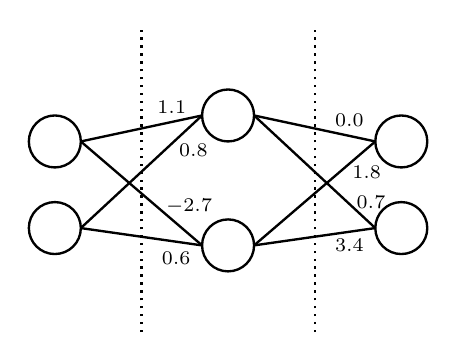
\begin{tikzpicture}[scale=1.1]
		% Input Layer
		\draw[line width=0.03cm] (0,0.2) circle (0.3);
		\draw[line width=0.03cm] (0,1.2) circle (0.3);
		% Hidden Layer
		\draw[line width=0.03cm] (2,0) circle (0.3);
		\draw[line width=0.03cm] (2,1.5) circle (0.3);
		% Output Layer
		\draw[line width=0.03cm] (4,0.2) circle (0.3);
		\draw[line width=0.03cm] (4,1.2) circle (0.3);
		
		% Dotted Lines
		\draw[line width=0.03cm,dotted] (1,-1) -- (1,2.5);
		\draw[line width=0.03cm,dotted] (3,-1) -- (3,2.5);
		
		% First Layer Lines
		\draw[line width=0.03cm] (0.3,1.2) -- (1.7,1.5);
		\draw[line width=0.03cm] (0.3,1.2) -- (1.7,0);
		\draw[line width=0.03cm] (0.3,0.2) -- (1.7,1.5);
		\draw[line width=0.03cm] (0.3,0.2) -- (1.7,0);
		
		% Second Layer Lines
		\draw[line width=0.03cm] (2.3,1.5) -- (3.7,1.2);
		\draw[line width=0.03cm] (2.3,1.5) -- (3.7,0.2);
		\draw[line width=0.03cm] (2.3,0) -- (3.7,1.2);
		\draw[line width=0.03cm] (2.3,0) -- (3.7,0.2);
		
		% Labels
		\node at (1.35,1.6) {\scriptsize$1.1$};
		\node at (1.6,1.1) {\scriptsize$0.8$};
		\node at (1.55,0.45) {\scriptsize$-2.7$};
		\node at (1.4,-0.15) {\scriptsize$0.6$};
		
		\node at (3.4,1.45) {\scriptsize$0.0$};
		\node at (3.6,0.85) {\scriptsize$1.8$};
		\node at (3.65,0.5) {\scriptsize$0.7$};
		\node at (3.4,0) {\scriptsize$3.4$};
		\end{tikzpicture}
		\]
	\end{enumerate} \pspace

\sol 
\begin{enumerate}[(a)]
\item {\itshape Solutions will vary.} \pspace

\item For ease of notation, we label our neural network as below:
		\[
		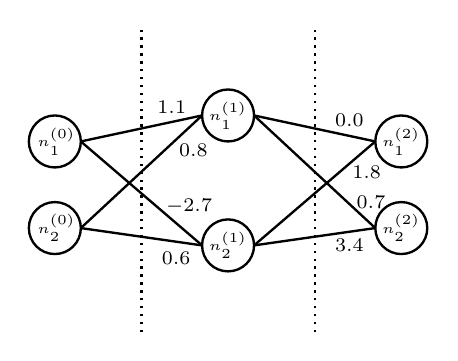
\begin{tikzpicture}[scale=1.1]
		% Input Layer
		\draw[line width=0.03cm] (0,0.2) circle (0.3);
		\draw[line width=0.03cm] (0,1.2) circle (0.3);
		
		% Hidden Layer
		\draw[line width=0.03cm] (2,0) circle (0.3);
		\draw[line width=0.03cm] (2,1.5) circle (0.3);
		
		% Output Layer
		\draw[line width=0.03cm] (4,0.2) circle (0.3);
		\draw[line width=0.03cm] (4,1.2) circle (0.3);
		
		% Dotted Lines
		\draw[line width=0.03cm,dotted] (1,-1) -- (1,2.5);
		\draw[line width=0.03cm,dotted] (3,-1) -- (3,2.5);
		
		% First Layer Lines
		\draw[line width=0.03cm] (0.3,1.2) -- (1.7,1.5);
		\draw[line width=0.03cm] (0.3,1.2) -- (1.7,0);
		\draw[line width=0.03cm] (0.3,0.2) -- (1.7,1.5);
		\draw[line width=0.03cm] (0.3,0.2) -- (1.7,0);
		
		% Second Layer Lines
		\draw[line width=0.03cm] (2.3,1.5) -- (3.7,1.2);
		\draw[line width=0.03cm] (2.3,1.5) -- (3.7,0.2);
		\draw[line width=0.03cm] (2.3,0) -- (3.7,1.2);
		\draw[line width=0.03cm] (2.3,0) -- (3.7,0.2);
		
		% Labels
		\node at (1.35,1.6) {\scriptsize$1.1$};
		\node at (1.6,1.1) {\scriptsize$0.8$};
		\node at (1.55,0.45) {\scriptsize$-2.7$};
		\node at (1.4,-0.15) {\scriptsize$0.6$};
		
		\node at (3.4,1.45) {\scriptsize$0.0$};
		\node at (3.6,0.85) {\scriptsize$1.8$};
		\node at (3.65,0.5) {\scriptsize$0.7$};
		\node at (3.4,0) {\scriptsize$3.4$};
		
		\node at (0.02,1.2) {\tiny$n^{(0)}_1$};
		\node at (0.02,0.2) {\tiny$n^{(0)}_2$};
		
		\node at (2,1.5) {\tiny$n^{(1)}_1$};
		\node at (2,0) {\tiny$n^{(1)}_2$};
		
		\node at (4,1.2) {\tiny$n^{(2)}_1$};
		\node at (4,0.2) {\tiny$n^{(2)}_2$};
		\end{tikzpicture}
		\]
We know that for $i \geq 1$, the `value' of each node is given by $\mathbf{n}_i= \sigma(W^{(i)} \mathbf{n}_{i-1} + \mathbf{b}_i)$, where $\mathbf{n}_i$ is the vector of the `values' for the $i$th node, $n^{(i)}_j$ is the $j$th entry of the $i$th node (that is $\mathbf{n}_i= (n^{(i)}_j)$), $W^{(i)}$ is the weight matrix (the transition matrix from $\mathbf{n}_{i-1}$ to $\mathbf{n}_i$, i.e. from the $(i-1)$th layer to the $i$th layer), $\mathbf{b}_i$ is the $i$th bias vector, and $\sigma$ is a choice of activation function (which we shall take to be the (logistic) sigmoid function $\sigma(x)= \frac{1}{1 + e^{-x}}$). Note that if $\mathbf{v}$ is a vector, $\sigma(\mathbf{v})$ is taken to mean $\mathbf{v}$ with $\sigma$ applied to each component. The matrix $W^{(i)}$ is given by $W^{(i)}= (w_{j,k})$, where $w_{j,k}$ is the weight from the $k$th node of the $(i-1)$th layer to the $j$th node of the $i$th layer.\footnote{We can derive this directly for this case. Observe that we must have $n^{(1)}_1= 1.1n^{(0)}_1 + 0.8n^{(0)}_2$ and $n^{(1)}_2= -2.7n^{(0)}_1 + 0.6n^{(0)}_2$. From this we can immediately see that $W^{(1)}= \begin{pmatrix} 1.1 & 0.8 \\ -2.7 & 0.6 \end{pmatrix}$.} In the notation of the video, we have $\mathbf{a}^{(i)}= \mathbf{n}^{(i)}$, $\mathbf{b}= \mathbf{b}_i$, and $W= W^{(i)}$. We have $\mathbf{n}^{(0)}= \mathbf{a}= \langle 3, -1, \rangle^T$. 
	\[
	\mathbf{n}^{(0)}= \mathbf{a}= \begin{pmatrix} 3 \\ -1 \end{pmatrix}
	\]
We can now compute the values of the nodes for the first layer:
	\[
	\begin{aligned}
	\mathbf{n}^{(1)}&= \sigma(W^{(1)} \mathbf{n}_0 + \mathbf{b}_1) \\[0.3cm]
	&= \sigma \left( 
	\begin{pmatrix} 
	1.1 & 0.8 \\
	-2.7 & 0.6
	\end{pmatrix}
	\begin{pmatrix} 3 \\ -1 \end{pmatrix} + \begin{pmatrix} 1.5 \\ -0.4 \end{pmatrix}
	\right) \\[0.3cm]
	&= \sigma \left( \begin{pmatrix} 2.5 \\ -8.7 \end{pmatrix} + \begin{pmatrix} 1.5 \\ -0.4 \end{pmatrix} \right) \\[0.3cm]
	&= \sigma \left( \begin{pmatrix} 4.0 \\ -9.1 \end{pmatrix} \right) \\[0.3cm]
	&= \begin{pmatrix} \sigma(4.0) \\ \sigma(-9.1) \end{pmatrix} \\[0.3cm]
	&= \begin{pmatrix} 0.982014 \\ 0.000111653 \end{pmatrix}
	\end{aligned}
	\]
We can then compute the output of the given neural network. 
	\[
	\begin{aligned}
	\mathbf{n}^{(2)}&= \sigma(W^{(2)} \mathbf{n}_1 + \mathbf{b}_2) \\[0.3cm]
	&= \sigma \left( 
	\begin{pmatrix} 
	0.0 & 1.8 \\
	0.7 & 3.4
	\end{pmatrix}
	\begin{pmatrix} 0.982014 \\ 0.000111653 \end{pmatrix} + \begin{pmatrix} 0.3 \\ 2.0 \end{pmatrix}
	\right) \\[0.3cm]
	&= \sigma \left( \begin{pmatrix} 0.000200975 \\ 0.687789 \end{pmatrix} + \begin{pmatrix} 0.3 \\ 2.0 \end{pmatrix} \right) \\[0.3cm]
	&= \sigma \left( \begin{pmatrix} 0.300200975 \\ 2.687789 \end{pmatrix} \right) \\[0.3cm]
	&= \begin{pmatrix} \sigma(0.300200975) \\ \sigma(2.687789) \end{pmatrix} \\[0.3cm]
	&= \begin{pmatrix} 0.574492 \\ 0.936302 \end{pmatrix}
	\end{aligned}
	\]
\end{enumerate}


\end{document}